\documentclass[12pt]{article}

\usepackage{sbc-template}
\usepackage{graphicx,url}
\usepackage[utf8]{inputenc}
\usepackage[T1]{fontenc}
\usepackage[colorlinks=true, allcolors=black]{hyperref}
\usepackage{booktabs}
\usepackage{longtable}
\usepackage{listings}
\usepackage{pgfplots}
\pgfplotsset{compat=1.18}
\lstset{breaklines=true, basicstyle=\ttfamily\small}

\sloppy

\title{\textbf{Auditoria Automática de Trabalhos Acadêmicos:\\
Alinhamento entre Promessas e Entregas com DoCO, TF-IDF e SciBERT}}

\author{João Pedro Tentis\inst{1}}

\address{PESC -- Universidade Federal do Rio de Janeiro (UFRJ)}

\begin{document}

\maketitle

\begin{abstract}
This paper presents a reproducible pipeline for auditing internal consistency in academic documents. The system extracts text from PDFs, segments rhetorical sections, assigns DoCO-compatible labels, compares introduction promises against delivery sections, and stores the resulting evidence for inspection. The work evolved from a heuristic baseline into an experimental protocol with provisional annotations, two similarity methods, formal ranking and classification metrics, and a SQLite database used by a command-line demonstration. The article reports the method, the experimental design, the observed limitations, and the next steps needed to turn the prototype into a more robust auditing tool.
\end{abstract}

\begin{resumo}
Este artigo apresenta um pipeline reprodutível para auditoria de consistência interna em trabalhos acadêmicos. O sistema extrai texto de PDFs, segmenta seções retóricas, atribui rótulos compatíveis com DoCO, compara promessas da introdução com seções de entrega e armazena as evidências geradas para inspeção. O trabalho evoluiu de um baseline heurístico para um protocolo experimental com anotações provisórias, dois métodos de similaridade, métricas formais de ranking e classificação, e um banco SQLite usado por uma demonstração em linha de comando. O artigo descreve o método, o desenho experimental, as limitações observadas e os próximos passos necessários para tornar o protótipo uma ferramenta de auditoria mais robusta.
\end{resumo}

\section{Links obrigatórios}

\begin{itemize}
    \item GitHub: \url{https://github.com/jtentis/projeto-BMT}
    \item Overleaf: \url{https://tinyurl.com/56nx8f4c}
\end{itemize}

\section{Introdução}

Trabalhos acadêmicos criam expectativas antes de apresentar resultados. A introdução declara objetivos, delimita o problema, antecipa contribuições e sugere quais lacunas o texto pretende preencher. Nas seções finais, o leitor espera encontrar uma resposta proporcional a essas promessas. Quando a conclusão extrapola os resultados, quando a seção de resultados não retoma o problema anunciado ou quando o escopo muda sem que a introdução acompanhe essa mudança, o documento perde consistência interna. A identificação desse desalinhamento costuma depender de leitura manual, conhecimento do domínio e atenção à estrutura retórica do texto.

O projeto BMT parte dessa motivação e propõe uma auditoria automática de alinhamento entre promessa e entrega. A proposta inicial definia três tarefas: extrair e segmentar documentos acadêmicos, rotular suas partes com um vocabulário compatível com a Document Components Ontology (DoCO) \cite{constantin2016doco}, e comparar os trechos de introdução com seções de resultados, discussão ou conclusão. A primeira entrega executável materializou essa proposta como um baseline offline: o sistema lia PDFs, extraía texto com \texttt{pypdf}, detectava cabeçalhos numerados e calculava similaridade TF-IDF com cosseno. As entregas seguintes estabilizaram o experimento: o dataset foi consolidado, as métricas foram formalizadas, os riscos de vazamento foram documentados e o relatório intermediário mostrou que o maior ganho naquele momento não era trocar de modelo, mas tornar o baseline auditável.

Na entrega final, o projeto avança em quatro pontos técnicos. Primeiro, o pipeline passa a exportar rótulos DoCO explícitos para as seções detectadas. Segundo, o experimento incorpora um ground truth provisório para permitir métricas formais de ranking e classificação. Terceiro, o baseline TF-IDF passa a ser comparado com um método baseado em SciBERT \cite{beltagy2019scibert}, modelo pré-treinado para textos científicos. Quarto, os resultados são persistidos em SQLite, permitindo consultas simples durante a demonstração. A contribuição do trabalho não está em substituir revisão humana, mas em produzir uma trilha reprodutível de evidências que ajude o avaliador a localizar documentos, seções e pares problemáticos.

\section{Trabalhos relacionados}

A primeira base conceitual do projeto é a representação de componentes documentais. A DoCO define um vocabulário estruturado para descrever partes de documentos, incluindo elementos estruturais e retóricos, como seção, parágrafo, introdução, discussão, figura e apêndice \cite{constantin2016doco}. Esse vocabulário não resolve sozinho a segmentação de PDFs, mas oferece uma forma comum de nomear a função das partes detectadas. No contexto deste projeto, a DoCO atua como camada semântica sobre uma segmentação heurística: o código ainda encontra cabeçalhos por padrões textuais, mas a saída passa a indicar explicitamente papéis como \texttt{doco:Introduction}, \texttt{doco:Results}, \texttt{doco:Discussion}, \texttt{doco:Methods} e \texttt{doco:Conclusion}.

O problema também se relaciona à classificação de zonas retóricas em artigos científicos. Teufel e Moens \cite{teufel2002summarizing} mostraram que o papel argumentativo de sentenças pode apoiar tarefas como sumarização científica. Liakata et al. \cite{liakata2010corpora} discutem corpora e avaliação para rotulação automática de artigos científicos, destacando que a estrutura retórica exige categorias funcionais e critérios de anotação consistentes. O presente trabalho não treina um classificador retórico supervisionado, mas herda dessa literatura a ideia de que a posição textual não basta: uma seção deve ser entendida pelo papel que exerce no argumento do documento.

Na dimensão de comparação textual, o baseline usa TF-IDF e similaridade do cosseno. Essa escolha segue uma tradição clássica de recuperação de informação, na qual termos ponderados por frequência local e raridade global formam uma representação vetorial simples e interpretável \cite{manning2008ir}. Como contraponto, o projeto usa SciBERT, um BERT treinado em corpus científico de larga escala, criado para melhorar tarefas de PLN em textos acadêmicos e técnicos \cite{beltagy2019scibert}. A comparação entre os dois métodos testa uma hipótese prática: uma representação contextual densa melhora a auditoria de alinhamento sem fine-tuning ou, neste cenário, a simplicidade lexical continua mais estável?

Por fim, as métricas de avaliação vêm da recuperação de informação e da classificação. Precision@k e MAP medem qualidade de ranking quando há julgamentos de relevância; NDCG incorpora relevância graduada e desconta posições mais baixas no ranking \cite{jarvelin2002cumulated}. Para a tarefa de alinhamento, essas métricas só fazem sentido depois da criação de um ground truth. Por isso as entregas anteriores tratavam Precision@k, MAP, NDCG e F1 como trabalho futuro. A versão final implementa esse elo: cada documento recebe anotações provisórias para os pares introdução-resultados e introdução-conclusão, permitindo avaliar os métodos de forma comparável.

\section{Método}

\subsection{Arquitetura do pipeline}

O pipeline executa seis etapas principais. A primeira lê todos os PDFs de \path{data/raw/} e registra metadados básicos, como nome do documento, número de páginas e status de processamento. A segunda extrai texto com \texttt{pypdf}. A terceira normaliza o texto, removendo hifenização artificial, padronizando espaços e criando uma versão sem acentos para busca de cabeçalhos. A quarta etapa identifica títulos numerados ou marcadores textuais próximos de introdução, métodos, resultados, discussão e conclusão. A quinta etapa converte essas seções para rótulos compatíveis com DoCO. A sexta etapa compara a seção de promessa, representada pela introdução, com seções candidatas de entrega.

Essa arquitetura preserva uma escolha importante feita no baseline: o sistema precisa continuar simples o suficiente para ser reproduzido localmente. A segmentação por cabeçalhos não é o método mais robusto para todos os PDFs, mas permite rastrear erros com facilidade. Cada documento gera texto extraído, texto normalizado, segmentação legada, seções DoCO, resultados de alinhamento e métricas. Assim, quando um score parece estranho, o avaliador consegue voltar ao trecho que originou a comparação. Essa rastreabilidade se mostrou essencial no relatório intermediário, especialmente no caso \texttt{LCMarques}, em que o score zero apontava mais para falha de segmentação do que para ausência comprovada de alinhamento.

\subsection{Rotulagem DoCO}

A proposta original previa uso do DoCO para representar as partes funcionais do documento. A versão final implementa essa decisão como uma camada explícita de rotulagem. Títulos associados a introdução recebem \texttt{doco:Introduction}; títulos associados a resultados, avaliação ou estudo de caso podem receber \texttt{doco:Results} ou \texttt{doco:Discussion}; títulos de conclusão recebem \texttt{doco:Conclusion}. O pipeline também reconhece seções de métodos e trabalhos relacionados quando os cabeçalhos permitem essa inferência. Essa rotulagem não deve ser lida como classificação perfeita: ela é uma aproximação baseada em regras, útil para padronizar a saída e preparar a substituição futura por um classificador retórico supervisionado.

O alinhamento usa a introdução como seção de promessa. As entregas candidatas são resultados, discussão e conclusão, com preservação dos nomes legados \texttt{results} e \texttt{conclusion} para compatibilidade com relatórios anteriores. Essa decisão reflete a formulação do problema nas entregas iniciais: não se busca medir qualidade científica global, mas verificar se aquilo que o texto promete no início reaparece nas partes em que o trabalho deveria entregar evidência, implementação, análise ou fechamento argumentativo.

\subsection{Métodos de similaridade}

O primeiro método é o baseline TF-IDF. Para cada par de trechos, o sistema cria vetores com n-gramas de tamanho 1 e 2 e calcula a similaridade do cosseno. O vocabulário é ajustado apenas nos trechos comparados dentro do próprio documento, evitando transferência de estatísticas entre documentos. Quando a segmentação produz trecho vazio ou texto sem vocabulário útil, o score é registrado como 0.0. Essa regra foi necessária após a ampliação do corpus, pois alguns PDFs novos geraram cabeçalhos de sumário como se fossem seções reais.

O segundo método usa SciBERT \cite{beltagy2019scibert}. O sistema carrega \path{allenai/scibert_scivocab_uncased}, tokeniza cada trecho, obtém os estados finais dos tokens válidos e calcula a média desses vetores. A similaridade entre promessa e entrega também usa cosseno. Essa implementação não aplica fine-tuning e não ajusta limiares por validação supervisionada. A comparação, portanto, avalia o comportamento de embeddings científicos prontos para uso em uma tarefa de alinhamento textual específica.

\subsection{Persistência e demonstração}

A entrega final adiciona uma etapa de exportação para SQLite. O banco \path{reports/final/results.db} contém tabelas para documentos, resultados por método, pares comparados, ground truth, métricas de ranking, métricas de classificação e avaliação por documento. Essa decisão atende a uma exigência prática da entrega: além dos arquivos CSV e JSON, o projeto oferece uma forma simples de consultar resultados com SQL. A demo CLI pode imprimir o resumo do corpus, a comparação entre TF-IDF e SciBERT, as métricas formais e o caso crítico \texttt{LCMarques} diretamente a partir do banco.

\section{Dados e protocolo experimental}

\subsection{Corpus}

O corpus atual contém 50 trabalhos acadêmicos em PDF coletados do Pantheon/UFRJ, repositório institucional mantido pelo Sistema de Bibliotecas e Informação da UFRJ. Os arquivos estão versionados em \path{data/raw/}, permitindo reprodução local sem nova coleta. O uso dos documentos tem finalidade acadêmica, experimental e reprodutível. As orientações do Pantheon indicam que o repositório participa do movimento de acesso aberto, preserva a produção acadêmica da UFRJ e respeita direitos autorais e eventuais embargos definidos pelas comunidades responsáveis.

O pipeline processou todos os 50 documentos sem erro de extração. O conjunto possui 3.595 páginas e 5.867.001 caracteres normalizados. A detecção automática encontrou introdução em 41 documentos, resultados em 40 e conclusão em 36. Esses números mostram uma diferença importante em relação à entrega de dados e métricas, que trabalhava com 10 documentos e cobertura completa das seções. Ao ampliar o corpus, o projeto ganhou diversidade, mas também expôs falhas de segmentação que não apareciam no conjunto menor.

\subsection{Ground truth provisório}

O arquivo \path{data/annotations/ground_truth.csv} contém 100 anotações, duas por documento: introdução para resultados e introdução para conclusão. Cada par recebe relevância graduada, com 0 para não relevante, 1 para parcialmente relevante e 2 para relevante. O arquivo também registra o alinhamento esperado em três classes: \texttt{aligned}, \texttt{partial} e \texttt{not\_aligned}. As anotações são provisórias e auditáveis. Elas permitem executar métricas formais, mas ainda não substituem um processo independente com dois avaliadores e medida de concordância.

Essa distinção metodológica importa. Nas entregas anteriores, o projeto evitava reportar F1, MAP ou NDCG porque não havia referência anotada. A versão final só calcula essas métricas depois de ligar os pares comparados a julgamentos de relevância. O ganho é experimental: agora TF-IDF e SciBERT podem ser comparados com a mesma referência. O limite também é claro: a qualidade da avaliação depende da qualidade futura dessas anotações.

\subsection{Controle de vazamento}

O experimento usa o corpus completo como conjunto fixo de avaliação. Não há divisão entre treino, validação e teste porque nenhum método foi treinado com os rótulos do corpus. O TF-IDF ajusta vocabulário apenas nos dois trechos comparados dentro de cada documento; o SciBERT usa pesos pré-treinados e não recebe fine-tuning; os limiares de rótulo são fixos. Como não há busca de hiperparâmetros guiada pelas métricas finais, o risco de vazamento fica concentrado na curadoria do ground truth e na interpretação dos resultados.

A validação cruzada também não foi usada. Ela faria sentido se o projeto treinasse um classificador ou calibrasse limiares com subconjuntos do corpus. Nesta etapa, a pergunta experimental é mais modesta: dado um corpus fixo, uma segmentação rastreável e duas funções de similaridade, quais pares recebem maior score e como esses scores se comportam contra as anotações disponíveis?

\section{Experimentos}

\subsection{Métricas}

Para ranking, o avaliador calcula Precision@1, Precision@2, AP, MAP, NDCG@1 e NDCG@2. Precision@k mede quantos itens relevantes aparecem até a posição k. AP resume a precisão ao longo das posições relevantes de um documento, e MAP calcula a média desses valores. NDCG usa a relevância graduada para premiar métodos que colocam pares mais relevantes no topo do ranking, seguindo a família de métricas proposta por Järvelin e Kekäläinen \cite{jarvelin2002cumulated}.

Para classificação, os scores são convertidos nos rótulos \texttt{aligned}, \texttt{partial} e \texttt{not\_aligned}. O pipeline usa dois limiares: scores maiores ou iguais a 0.35 indicam alinhamento; scores entre 0.15 e 0.35 indicam alinhamento parcial; scores abaixo de 0.15 indicam não alinhamento. O avaliador calcula acurácia, precisão macro, revocação macro, F1 e macro-F1. Esses valores devem ser lidos junto com a natureza provisória do ground truth e com a presença de documentos sem seções suficientes.

\subsection{Resultados agregados}

\begin{table}[h]
    \centering
    \begin{tabular}{lrrrrr}
        \toprule
        Método & P@1 & P@2 & MAP & NDCG@1 & NDCG@2 \\
        \midrule
        TF-IDF & 0.5200 & 0.4700 & 0.5200 & 0.5200 & 0.5200 \\
        SciBERT & 0.5000 & 0.4700 & 0.5100 & 0.4600 & 0.5004 \\
        \bottomrule
    \end{tabular}
    \caption{Métricas de ranking no corpus com 50 documentos.}
    \label{tab:ranking}
\end{table}

\begin{table}[h]
    \centering
    \begin{tabular}{lrrrrr}
        \toprule
        Método & Acurácia & Precisão & Revocação & F1 & Macro-F1 \\
        \midrule
        TF-IDF & 0.9333 & 0.9015 & 0.9327 & 0.9144 & 0.9144 \\
        SciBERT & 0.5067 & 0.5098 & 0.3571 & 0.2752 & 0.2752 \\
        \bottomrule
    \end{tabular}
    \caption{Métricas de classificação para os pares anotados.}
    \label{tab:classificacao}
\end{table}

Os resultados de ranking ficaram próximos, com vantagem pequena para TF-IDF. Em classificação, a diferença foi maior: o TF-IDF se ajustou melhor aos limiares atuais, enquanto o SciBERT atribuiu scores altos a muitos pares que o ground truth provisório trata como parciais ou não alinhados. Esse comportamento confirma uma hipótese levantada no relatório intermediário: usar uma representação semântica mais forte não resolve, por si só, problemas de segmentação, calibração e definição de relevância.

\begin{figure}[h]
    \centering
    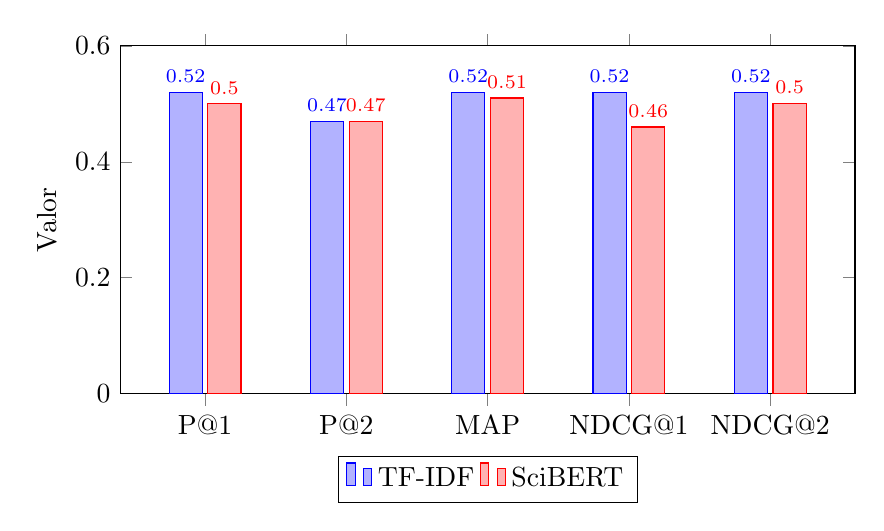
\begin{tikzpicture}
        \begin{axis}[
            ybar,
            width=0.9\linewidth,
            height=6cm,
            ymin=0,
            ymax=0.6,
            ylabel={Valor},
            symbolic x coords={P@1,P@2,MAP,NDCG@1,NDCG@2},
            xtick=data,
            bar width=12pt,
            enlarge x limits=0.15,
            legend style={at={(0.5,-0.18)}, anchor=north, legend columns=2},
            nodes near coords,
            nodes near coords style={font=\scriptsize},
        ]
            \addplot coordinates {(P@1,0.52) (P@2,0.47) (MAP,0.52) (NDCG@1,0.52) (NDCG@2,0.52)};
            \addplot coordinates {(P@1,0.50) (P@2,0.47) (MAP,0.51) (NDCG@1,0.46) (NDCG@2,0.5004)};
            \legend{TF-IDF,SciBERT}
        \end{axis}
    \end{tikzpicture}
    \caption{Comparação visual das métricas de ranking entre TF-IDF e SciBERT.}
    \label{fig:ranking}
\end{figure}

\begin{table}[h]
    \centering
    \begin{tabular}{lr}
        \toprule
        Rótulo TF-IDF & Documentos \\
        \midrule
        \texttt{high} & 24 \\
        \texttt{medium} & 2 \\
        \texttt{low} & 14 \\
        \texttt{insufficient\_sections} & 10 \\
        \bottomrule
    \end{tabular}
    \caption{Distribuição dos rótulos de alinhamento no corpus ampliado.}
    \label{tab:distribuicao}
\end{table}

\begin{figure}[h]
    \centering
    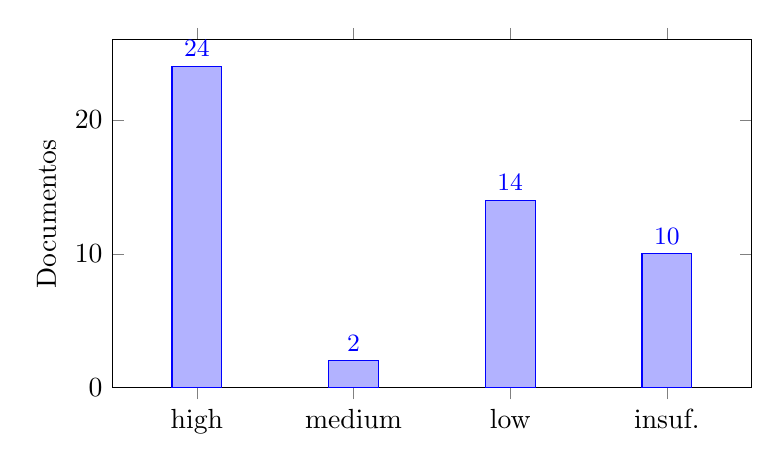
\begin{tikzpicture}
        \begin{axis}[
            ybar,
            width=0.8\linewidth,
            height=6cm,
            ymin=0,
            ymax=26,
            ylabel={Documentos},
            symbolic x coords={high,medium,low,insuf.},
            xtick=data,
            bar width=18pt,
            enlarge x limits=0.18,
            nodes near coords,
            nodes near coords style={font=\small},
        ]
            \addplot coordinates {(high,24) (medium,2) (low,14) (insuf.,10)};
        \end{axis}
    \end{tikzpicture}
    \caption{Distribuição dos rótulos TF-IDF no corpus com 50 documentos.}
    \label{fig:labels}
\end{figure}

\begin{longtable}{p{0.28\linewidth}rp{0.18\linewidth}rp{0.18\linewidth}}
    \caption{Casos representativos da comparação por documento.} \label{tab:comparacao_documento} \\
    \toprule
    Documento & TF-IDF & Rótulo & SciBERT & Rótulo \\
    \midrule
    \endfirsthead
    \toprule
    Documento & TF-IDF & Rótulo & SciBERT & Rótulo \\
    \midrule
    \endhead
    AMDavid & 0.4040 & high & 0.9690 & high \\
    BCAbreu & 0.4981 & high & 0.9745 & high \\
    GMGonçalves & 0.7399 & high & 0.9451 & high \\
    LCMarques & 0.0000 & low & 0.6965 & high \\
    LFSuett & 0.0000 & insuff. & 0.0000 & insuff. \\
    MBSTavares & 0.0064 & low & 0.5668 & high \\
    NSahlit & 0.0000 & low & 0.3118 & medium \\
    PVMNascimento & 0.4224 & high & 0.9748 & high \\
    TAGurgel & 0.0612 & low & 0.6679 & high \\
    monopoli10015726 & 0.0000 & low & 0.1441 & low \\
    \bottomrule
\end{longtable}

\section{Discussão}

O resultado mais importante não é a vitória de um método sobre outro, mas a separação entre três fontes de erro. A primeira fonte está na extração e segmentação: quando o PDF produz sumário como texto de seção, cabeçalhos duplicados ou trechos vazios, qualquer método de similaridade recebe entrada ruim. A segunda fonte está na representação textual: TF-IDF mede sobreposição lexical e perde casos em que a entrega usa vocabulário diferente da promessa; SciBERT aproxima textos científicos longos de forma ampla e, sem calibração, tende a superestimar alinhamento. A terceira fonte está no próprio ground truth, que ainda é provisório e precisa de revisão independente.

O caso \texttt{LCMarques} mostra como esses erros se combinam. No corpus de 10 documentos, ele já aparecia como o caso crítico, com score TF-IDF igual a 0.0000. No corpus ampliado, o SciBERT atribuiu 0.6965 ao mesmo documento, produzindo leitura oposta. A inspeção dos artefatos indica que a introdução extraída contém ruído de sumário. Assim, o desacordo entre métodos funciona como sinal de auditoria: quando um método lexical vê zero e um embedding contextual vê alto alinhamento, o avaliador deve verificar primeiro a seção comparada, não concluir que um dos métodos ``entendeu'' melhor o texto.

A ampliação do corpus também muda a interpretação da cobertura. Com 10 PDFs, todos os documentos tinham introdução, resultados e conclusão detectados. Com 50 PDFs, a diversidade editorial aumentou e a cobertura caiu. Isso não invalida o pipeline; pelo contrário, mostra que a avaliação deixou de operar apenas em casos convenientes. A partir desse ponto, melhorar segmentação passa a ser tão importante quanto testar modelos mais sofisticados.

\subsection{Ameaças à validade}

A validade interna depende da qualidade da segmentação. O pipeline compara seções inteiras, não sentenças anotadas manualmente, e por isso um limite de seção mal posicionado altera o score final. A validade de construto depende da definição de alinhamento: relevância lexical, retomada semântica e consistência argumentativa não são a mesma coisa. O ground truth provisório aproxima esses conceitos para viabilizar avaliação formal, mas ainda precisa de instruções de anotação mais rigorosas e revisão por mais de um avaliador.

A validade externa também tem limites. O corpus cresceu para 50 documentos, mas continua concentrado em uma fonte institucional e em trabalhos acadêmicos com formatos heterogêneos. A generalização para outros repositórios, áreas e estilos editoriais exige nova coleta e nova auditoria. Além disso, o SciBERT foi treinado majoritariamente em literatura científica em inglês; seu uso em trabalhos em português pode preservar algumas regularidades científicas, mas não garante representação ideal para o idioma e o domínio local.

\section{Conclusão e trabalhos futuros}

O projeto entregou um pipeline reprodutível para auditar alinhamento entre promessas e entregas em trabalhos acadêmicos. A trajetória das entregas mostra uma evolução incremental: a proposta definiu o problema e o uso do DoCO; o baseline criou uma execução mínima; a entrega de dados e métricas estabilizou o protocolo; o relatório intermediário identificou limitações concretas; a versão final adicionou ground truth provisório, SciBERT, métricas formais, SQLite e demo. Essa sequência importa porque impediu que a comparação de modelos escondesse problemas básicos de corpus, segmentação e avaliação.

Como próximos passos, o projeto deve revisar manualmente as segmentações dos documentos com \texttt{insufficient\_sections}, criar anotação independente com medida de concordância, calibrar limiares separadamente para TF-IDF e SciBERT, e testar modelos ajustados ao português acadêmico. A substituição gradual da segmentação por cabeçalhos por um classificador retórico supervisionado é o caminho mais promissor. Sem essa melhoria, modelos mais fortes continuarão comparando trechos que nem sempre correspondem às funções retóricas pretendidas.

\appendix

\section{Uso de IA}

O autor usou Codex/ChatGPT para planejar etapas, revisar texto, apoiar a implementação, estruturar relatórios e conferir comandos de validação. O autor manteve sob responsabilidade humana as decisões de escopo, execução, validação, interpretação dos resultados e submissão. A IA apoiou a organização do ground truth provisório, mas não deve ser tratada como fonte autônoma de verdade experimental. As anotações exigem auditoria humana independente antes de uso como referência definitiva.

\begin{thebibliography}{9}

\bibitem{beltagy2019scibert}
Beltagy, I., Lo, K., and Cohan, A. (2019).
\newblock SciBERT: A Pretrained Language Model for Scientific Text.
\newblock In \textit{Proceedings of EMNLP-IJCNLP}, pages 3615--3620.
\newblock \url{https://arxiv.org/abs/1903.10676}.

\bibitem{constantin2016doco}
Constantin, A., Peroni, S., Pettifer, S., Shotton, D., and Vitali, F. (2016).
\newblock The Document Components Ontology (DoCO).
\newblock \textit{Semantic Web}, 7(2):167--181.
\newblock \url{https://www.semantic-web-journal.net/content/document-components-ontology-doco}.

\bibitem{jarvelin2002cumulated}
Järvelin, K. and Kekäläinen, J. (2002).
\newblock Cumulated Gain-Based Evaluation of IR Techniques.
\newblock \textit{ACM Transactions on Information Systems}, 20(4):422--446.
\newblock \url{https://doi.org/10.1145/582415.582418}.

\bibitem{liakata2010corpora}
Liakata, M., Teufel, S., Siddharthan, A., and Batchelor, C. R. (2010).
\newblock Corpora for the Conceptualisation and Zoning of Scientific Papers.
\newblock In \textit{Proceedings of LREC}.

\bibitem{manning2008ir}
Manning, C. D., Raghavan, P., and Schütze, H. (2008).
\newblock \textit{Introduction to Information Retrieval}.
\newblock Cambridge University Press.
\newblock \url{https://nlp.stanford.edu/IR-book/}.

\bibitem{teufel2002summarizing}
Teufel, S. and Moens, M. (2002).
\newblock Summarizing Scientific Articles: Experiments with Relevance and Rhetorical Status.
\newblock \textit{Computational Linguistics}, 28(4):409--445.

\end{thebibliography}

\end{document}
